%%%%%%%%%%%%%%%%%%%%%%%%%%%%%%%%%%%%%%%%%%%%%%%%%%%%%%%%%%%%%%%%%%%%%%%%%%%%%%%%%%%%%%%%%%%%%%%%%%%%%%%%%%%%%%%%%%%%%%%%%%%%%%%%%
\chapter{On the Client Side}
\label{cha:on_the_client_side}

%%%%%%%%%%%%%%%%%%%%%%%%%%%%%%%%%%%%%%%%%%%%%%%%%%%%%
\section{The iPhone}
\label{sec:the_iphone}

\subsection{The Device}
The iPhone is a last generation smartphone developed by Apple and was revealed for the first time in 2007. It features advanced functionalities such as multimedia support, internet access, video games and many more. Up to this day, forty-two millions iPhone have been sold across the globe.\\

Its main characteristic is that its User Interface (UI) is almost only based on two inputs:
\begin{itemize}
\item{a large multi-touch screen}
\item{a 3-axis accelerometers}
\end{itemize}
As such, the iPhone does not possess any physical keyboard. Instead, a virtual keyboard can be summoned any time it is necessary, leaving a larger screen for applications.\\

The last generation of iPhone, the iPhone 3G-S, also includes a GPS, a compass, and a 3-megapixels camera, which seems to make it a perfect candidate for any Augmented Reality application. Unfortunately, the pragmatic access to the camera is not yet fully available, so image recognition is not yet an option, thought an upcoming version of its Operating System (OS) will allow the access to the video data of the camera.\\

In order to install new applications on an iPhone, one must download it from the AppStore, the internet-based retail store from Apple for iPhones, iPods and the iPad. Apple having a highly proprietary policy on its product, this is actually the only way to distribute iPhone applications.

\subsection{The Development Tools}

To develop an application for iPhone, a specific Framework is required. We will have a look at its nature in this section.

\subsubsection{Objective-C}

First of all, any software developed for iPhone must be programmed in Objective-C, although it is possible to call C and C++ functions from code.\\

Objective-C is an Object-Oriented (OO) reflexive programming language build upon the C language. It is comparable to C++ from this perspective, but differs greatly in many ways, especially in its dynamic message passing system, in being weakly typed and in being able to perform dynamic loading. In its latest version, Objective-C also features a Garbage Collector which subtracts the programmer from advanced memory management considerations. Unfortunately, this feature is not available for iPhone development.\\

As mentioned above, one of the interesting features of Objective-C is its message passing in lieu of method call for an object. In Objective-C terminology, calling a Method from an Object consists instead of sending a Message to a Receiver. The following example send a message "say" with parameter @"hello world!"  to the receiver named "receiver", and the answer "result" is of type "BOOL".

\parbox{15cm}{
\begin{Verbatim}[commandchars=@\[\]]
@PYaJ[BOOL] result @PYbf[=] @PYZlb[]receiver @PYai[say:]@PYad[@PYZat[]"]@PYad[hello world!]@PYad["]@PYZrb[];
\end{Verbatim}

}

This is very close to the elegant Smalltalk messaging system. In practice, the Receiver is an object "id", which is similar to an anonymous pointer to an object. When messaging a receiver, the object sending a message does not need to know if the object it is sending to will be able to handle its request or not. This is really convenient since the sender does not need to be aware of the receiver. This system allows complex interactions between object.

\subsubsection{iPhone SDK}

In order to compile code for the iPhone, the use of Xcode as Integrated Development Environment is almost unavoidable. Apple has a highly proprietary approach for its products, and programming for an Apple environment is much restrictive to this regard. Fortunately, Xcode and the set of tools provided by Apple offer a great comfort of use in many cases, especially for debugging, or for creating interfaces with the use of the Interface Builder (IB).\\

Once Xcode is set up, the iPhone Software Development Kit must be installed on Xcode. The iPhone SDK takes advantage of all the features of Xcode, including its set of external tool to the largest extent. After being registered to the iPhone developer's program, Xcode can also be linked directly to an actual iPhone device in order to test an application in real-time with any monitoring tool available.\\

This SDK contains Application Programming Interfaces (API) to all the accessible libraries of the iPhone, including Cocoa. Unfortunately, many functionalities such as the access to raw data from the video camera are not part of a public API, so their libraries are considered as not accessible and therefore their use are forbidden by Apple.

%%%%%%%%%%%%%%%%%%%%%%%%%%%%%%%%%%%%%%%%%%%%%%%%%%%%%
\section{The Application}
\label{sec:the_application}

\subsection{What it does}

This application has been designed for travellers in Sweden that are looking for a nearby public transport station. Augmented Reality makes it very intuitive to find a nearby stop: the user just has to "look around" with his iPhone, and the closest stops will appear at their positions. When the user holds his iPhone in one direction, a virtual Map is projected on the estimated ground, and on it a set of three-dimensional pins indicating nearby stops. All this is done in realtime and fits the position of the iPhone with six degrees of movements.\\

To make it even easier for the user, a flat Google Map is available when the device is held horizontally. The flat map also displays pins representing the nearby stops. The Map is always oriented in the direction of the user for more convenience. This can be useful when directions are required. \\

If the user press a pin in either Augmented Reality or Flat Map, a bubble will appear with the stop name, its distance from the user and the Bus/Tram/Boat/Subway line numbers it serves. If this stop is interesting to him, the user can check the next departures by pressing the arrow in the bubble.\\

The application flips horizontally and displays the next departures in a scrollable view, with indexes on the side for quick navigation. This is a really efficient way to check for the next departures: only two "clicks" are required to access the desired data.\\

Augmented Reality makes the application very interesting for people that are uncomfortable at reading maps when discovering a new city.\\

But this application has also been designed for people that are already familiar with the city they visit. Simply by pointing at a stop they are interested in, they can get the next departures without wasting their time by going to a stop in order to consult its timetable.\\

For now, the application is available for Göteborg and Stockholm, with their respective public transport companies Västtrafik and Storstockholms Lokaltrafik. But additional providers could be added later on.\\

The application is available in English, Swedish, French and Chinese and can be downloaded from the AppStore under the name "Hållplats SE".

\subsection{How it works}

The application takes advantage of the GPS capabilities of the iPhone to locate the user on a map. Then thanks to the compass, we are able to estimate the direction he is looking at, and the 3-axis accelerometer allows us to evaluate the angle at which he holds his phone. Note that this application requires a GPS and a compass, and therefore is only compatible with the iPhone 3G-S.\\

Built-in APIs makes it easy to access the accelerometer, compass and GPS data. When an update to either of these sensors is generated, a message is sent to their respective delegates in a way that could be compared to Events in Java.\\

Once the position of the user is known, a request is made over the internet to determine the bus stops that are close to him. The answer to this request will be a list of stops with their names and locations together with a forecast list for each of them.\\

An item in the forecast list is composed of a line number, a destination and a set of attributes indicating the time of departure plus some information on the quality of the travel.\\

Once the positions of the bus stops are known, we can project them in the virtual space according to the user's coordinates, heading direction and phone holding angle. Our implementation of Augmented Reality hence follows the second method defined in Section \ref{sec:how_does_ar_work}: we use sensors to know the position of the camera in a known space.\\

To cope with the precision errors of acceleration and heading measurement, a buffer is used to get the average values on an arbitrary period of time before updating the knowledge on the user's position. Animations are also used to make transitions between two views appear smoother.

%%%%%%%%%%%%%%%%%%%%%%%%%%%%%%%%%%%%%%%%%%%%%%%%%%%%%
\section{Implementation of the Augmented Reality View}
\label{sec:implementation_of_ar_view}

\subsection{View Hierarchy}

\begin{figure}[ht]
\center
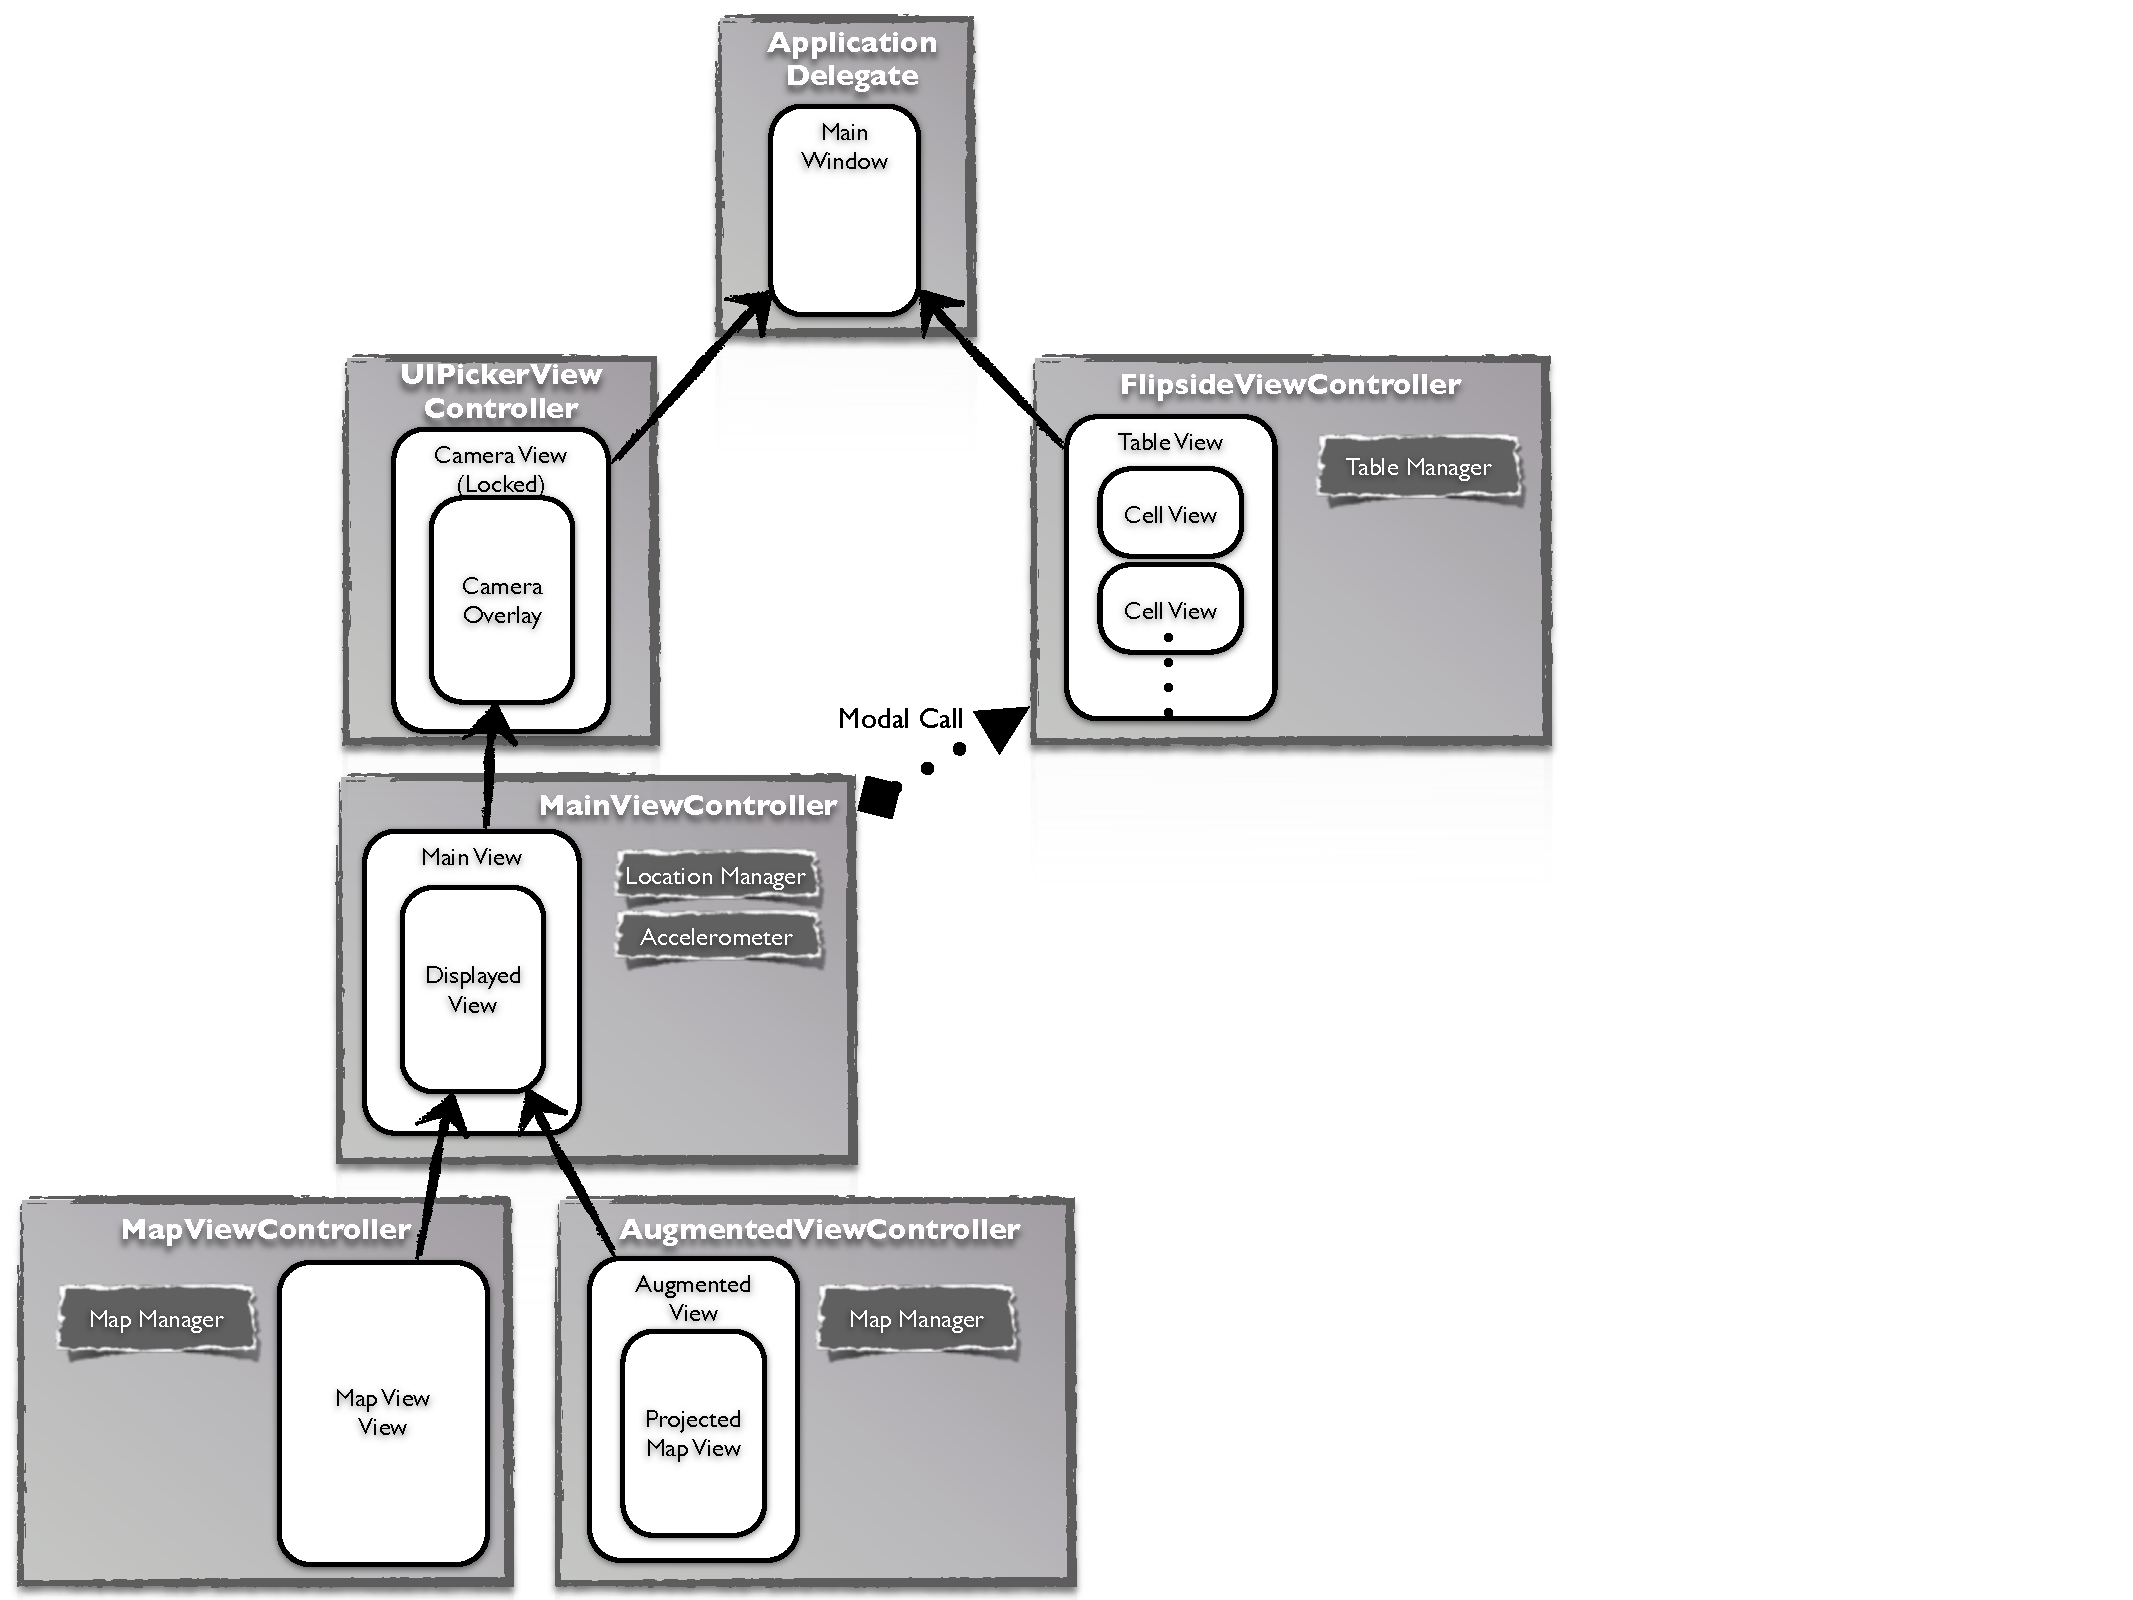
\includegraphics[scale=0.5]{pics/client_view_hierarchy}
\caption{Scheme of the View Hierarchy of the application}
\label{fig:client_view_hierarchy}
\end{figure}

When developing for iPhone, the Model-View-Controller (MVC) is the best architecture to go with. There are well defined classes for views and controllers in the Cocoa environment, so we took advantage of that when designing our application.\\

When using the Cocoa environment, each view must be a subclass of the UIView class, and each controller of the UIViewController class. A view is automatically linked to a view controller.\\

A view can contain other views that will be considered as its subviews, and each view has a frame in which it renders itself. Views can have transparent or semi-transparent backgrounds, so it is possible to create a complex view hierarchy without hassle.\\

Figure \ref{fig:client_view_hierarchy} shows the view hierarchy for our application.\\

In order to render a view on screen, one must define an application window that is a subclass of UIWindow and that will take care of rendering every visible view on the iPhone's screen. By definition, a UIWindow must be the higher node in any view hierarchy.\\

Before further considerations, one should know that there is a serious restriction on the iPhone SDK up to the version 3.2 which prohibits to insert a camera view (UIImagePickerView) as a subview to a UIView. Instead, it must be directly put into a UIWindow. Since we want to use the camera in our application, we have no choice but to put it on top of our view stack. This is semantically very wrong, but there are no alternatives left here by Apple.\\

Furthermore, the camera view itself is locked, so we can't help but use a view called "Camera Overlay" to display any view on top of it. That is ugly and clearly opposed to the concept of our application, but again there is no other way to do it.\\

As a result, the camera is always rendering in the background of our application, and everything else is rendered on top of it.\\

Now we have a window and a background with a camera view, and we want to be able to switch between a Map View and an Augmented Reality View. To do so, we implement a Main View that will display either of them according to the iPhone position. In order to avoid redundancy, all the data of the application is handled by the Main View Controller and dispatched in its subview, be it a Map View or an Augmented View. The same goes for the acceleration and location data.\\

To present the forecast of a stop, a "modal view" is opened by the Main View Controller.  The display of a modal view will replace the content of the actual window by a temporary view. When dismissing this view, the previous content of the window is loaded again and the application continues.\\

This modal view is a table view itself composed of view cells that are respectively subclasses of UITableView and UITableViewCell. Those view cells are used to display the forecasts list for a bus stop.

\subsection{Positioning within 6 degrees of freedom}

In our application, we need to locate the camera of the iPhone within 6 degrees of freedom:

\begin{itemize}
\item{Latitude ($\varphi$)}
\item{Longitude ($\lambda$)}
\item{Altitude}
\item{Azimuth ($\theta$)}
\item{Roll angle ($\alpha$)}
\item{Pitch angle ($\beta$)}
\end{itemize}

Those degrees of freedom are illustrated in Figure \ref{fig:iphone_orientation}.

\begin{figure}[ht]
\center
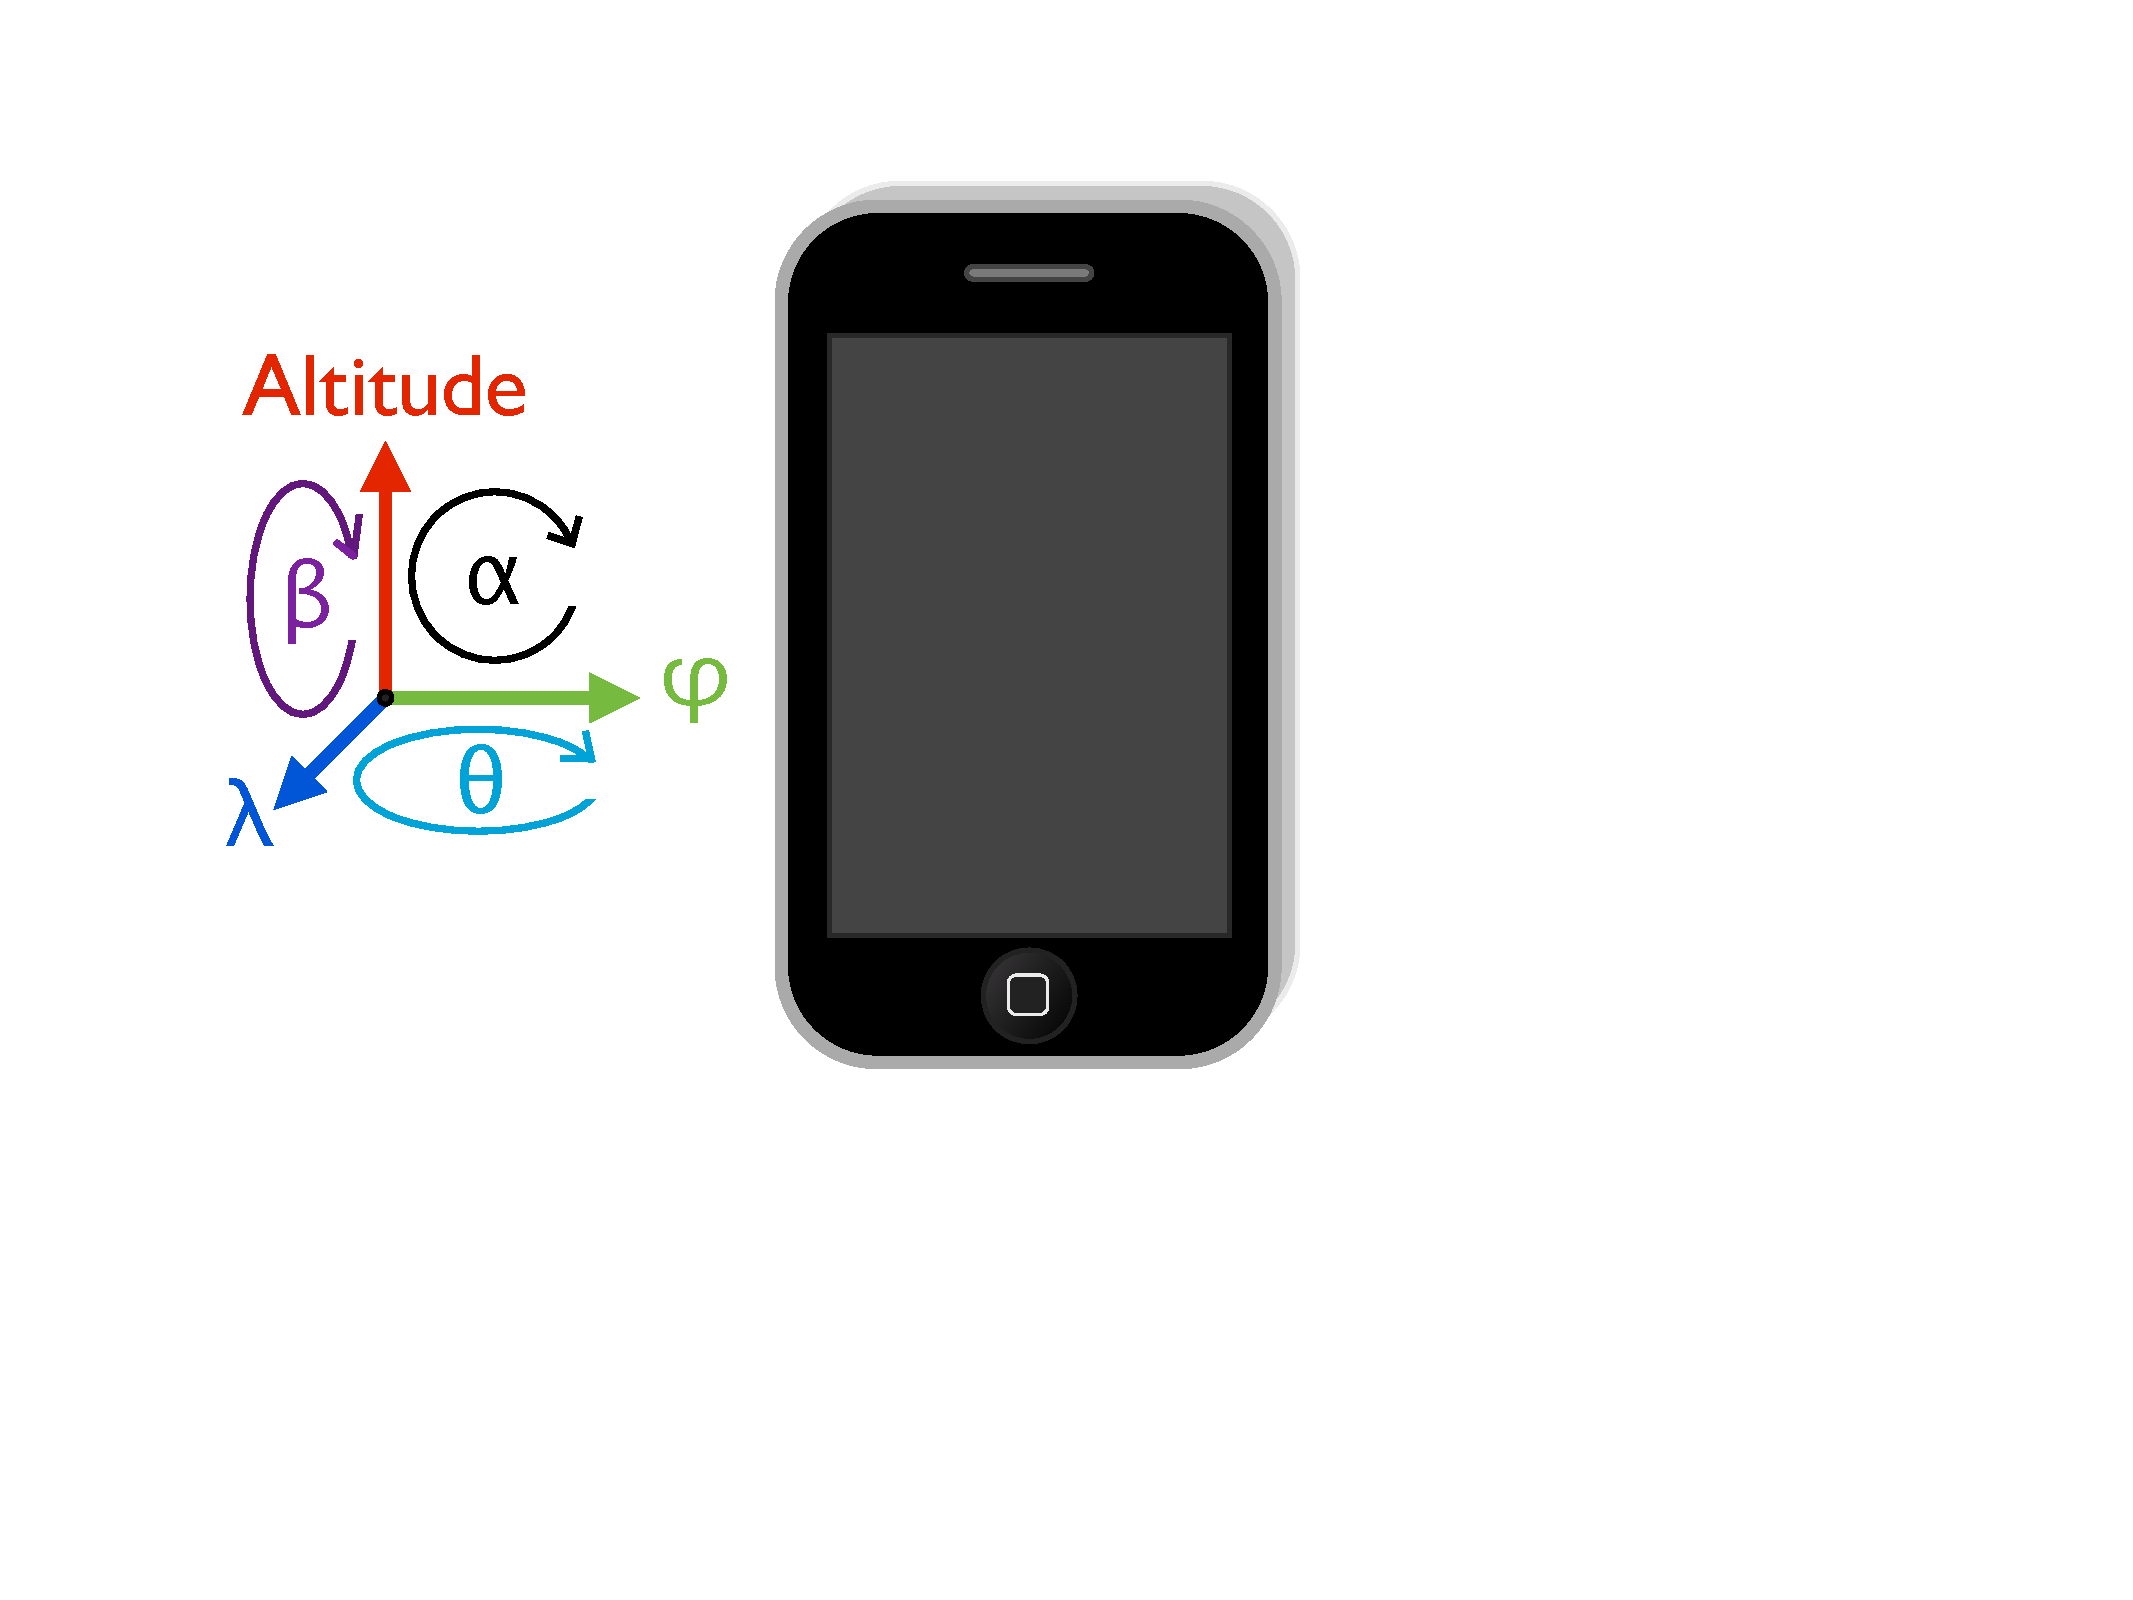
\includegraphics[scale=0.5]{pics/iphone_orientation}
\caption{the 6 degrees of freedom of the iPhone}
\label{fig:iphone_orientation}
\end{figure}

The GPS directly gives us the Altitude, Latitude and Longitude of the user whereas the compass gives us his Azimuth. This directly takes care of 4 out of the 6 degrees.\\

But thanks to the 3-axis accelerometer, the roll angle and pitch angle can easily be computed by the mean of simple trigonometry as shown in Figure \ref{fig:six_degrees_angles}

\begin{figure}[ht]
\center
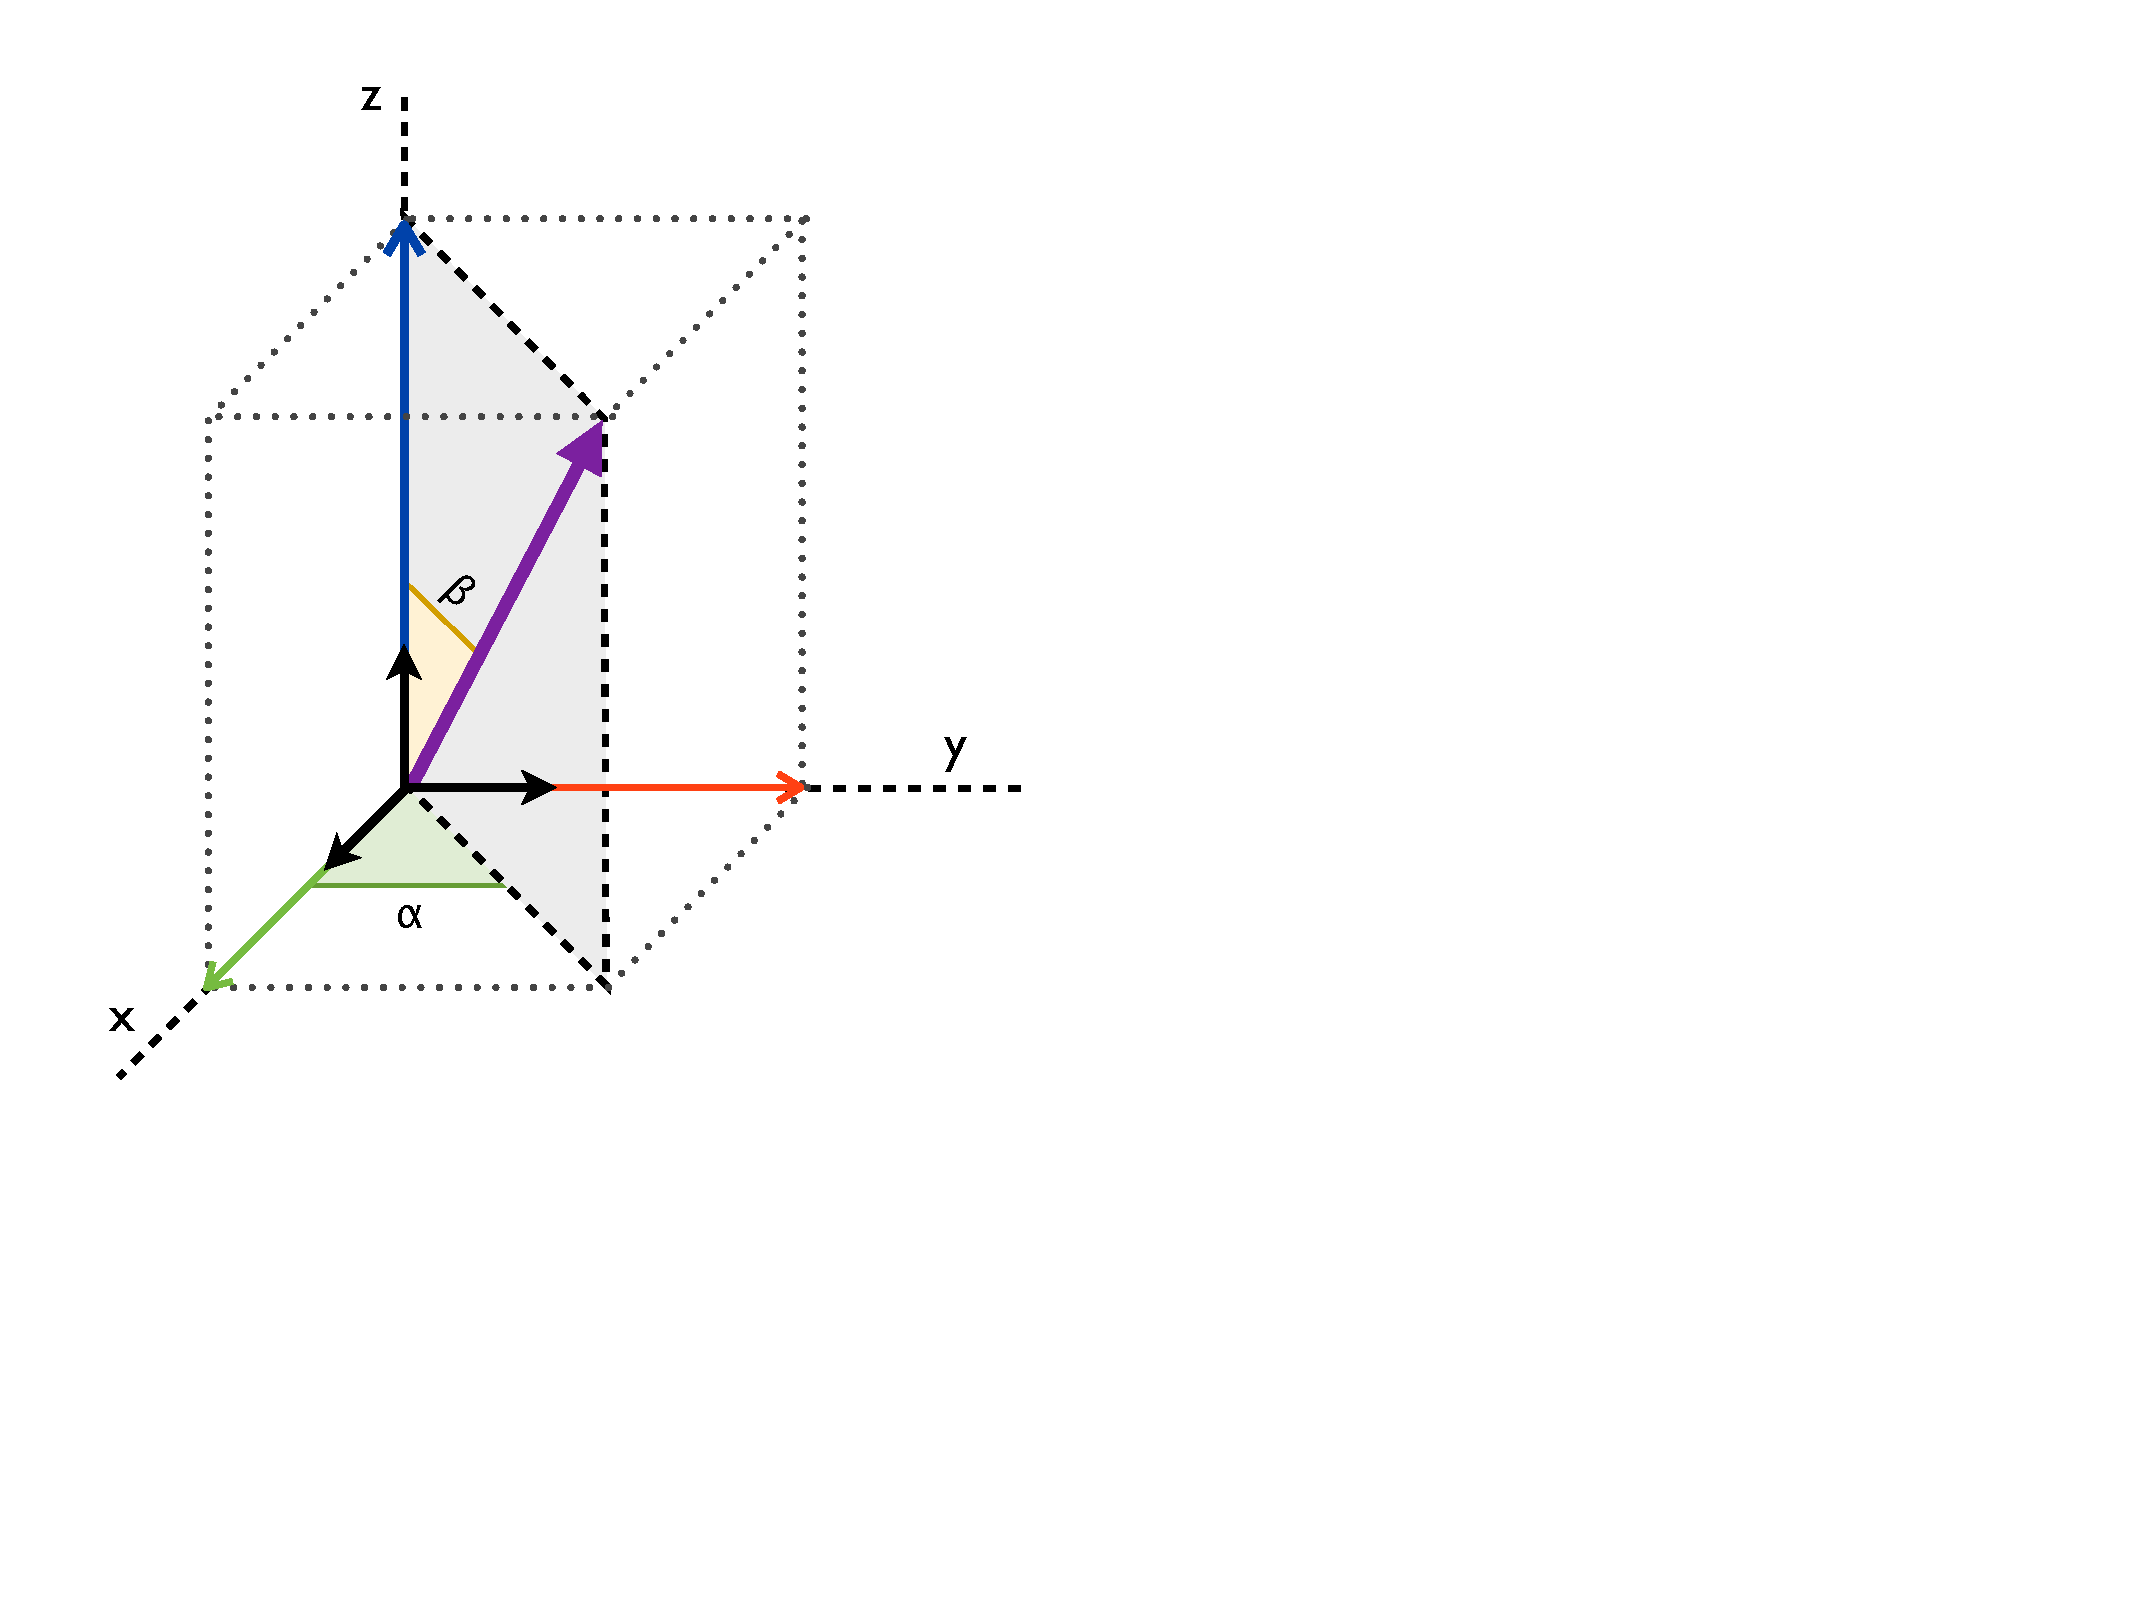
\includegraphics[scale=0.5]{pics/six_degrees_angles}
\caption{Projection giving the Roll and Pitch angles, respectively $\alpha$ and $\beta$}
\label{fig:six_degrees_angles}
\end{figure}

To compute $\alpha$ and $\beta$, we use the following equations:

\[\alpha = \textrm{atan2}(x, y)\]
\[\beta = \textrm{atan2}(\sqrt{y^2+x^2}, z)\]

Where $x$, $y$ and $z$ are respectively the accelerations values on the X-, Y- and Z-axis an atan2($a${},{}$b$) is a function that gives the angle in radians between a vector ($a$ , $b$) and the X-axis.

\subsection{3D Projection}

Now that we know the position of the camera relatively to the object we want to display, we must use our knowledge to render the Augmented View.\\

\subsubsection{Rendering the ground Map}

First, we project a Map on the plane defining the ground. The iPhone has an API to perform 3D projections, by the mean of layer transformations. To apply a transform to a layer, one must provide the transform matrix corresponding to the desired projection.\\

In this case, the transformation will be a rotation of $\psi = \pi/2$ on the X-axis and another $\theta$ corresponding to the Azimuth on the Y-Axis, followed by translations $t_y$ and $t_z$ on the Y and Z axis to give depth to the view, which gives the following matrix:\\

\[ \left( \begin{array}{cccc}
	\textrm{cos} \theta 				& 0 					& -\textrm{sin} \theta 				& - \textrm{sin} \theta / e_z\\
	\textrm{sin} \psi \textrm{ sin} \theta 	& \textrm{cos} \psi		& \textrm{sin} \psi \textrm{ cos} \theta 	& \textrm{sin} \psi \textrm{ cos} \theta  / e_z\\
	\textrm{cos} \psi \textrm{ sin} \theta	& -\textrm{sin} \psi		& \textrm{cos} \psi \textrm{ cos} \theta	& \textrm{cos} \psi \textrm{ cos} \theta / e_z\\
	0							& t_y					& t_z 							& t_z / e_z
\end{array} \right)\]\\

where $e_z$ is the distance of the user from the projection plan. Since we have $\psi = \pi / 2$, the transformation matrix becomes: \\

\[ \left( \begin{array}{cccc}
	\textrm{cos} \theta	& 0 				& -\textrm{sin} \theta 	& - \textrm{sin} \theta / e_z\\
	\textrm{sin} \theta 	& 0				& \textrm{cos} \theta 		& \textrm{cos} \theta  / e_z\\
	0				& -1				& 0					& 0\\
	0				& t_y				& t_z 				& t_z / e_z
\end{array} \right)\]\\

\subsubsection{Rendering the bus stops}

Once the map is projected on the proper plane, we can project the buttons representing the bus stops. First, we need to compute the distance and the azimuth of the stop relatively to the camera.\\

To compute the distance $d$, we use a simplified version of the great-circle formula as shown in Equation \ref{equ:great_circle_projection} where $\varphi_s$ and $\lambda_s$ are the Latitude and Longitude of the standpoint (camera position), $\varphi_f$ and $\lambda_f$ the ones of the forepoint (bus stop location) and $R$ is the average radius of Earth ($\approx6371$km).

\begin{equation}
\label{equ:great_circle_projection}
d =  R \times \textrm{arccos}\left(\textrm{sin}\varphi_s \textrm{ sin}\varphi_f + \textrm{cos}\varphi_s \textrm{ cos}\varphi_f \textrm{ cos}(\lambda_f-\lambda_s)\right)
\end{equation}

To compute the relative azimuth $\theta_r$, we use the formula shown in Equation \ref{equ:azimuth}. In this formula, atan2($x${},{}$y$) is a function that gives the angle in radians between the vector ($x$ , $y$) and the X-axis.

\begin{equation}
\label{equ:azimuth}
\theta_r = \textrm{atan2}\left(\textrm{sin}( \lambda_f - \lambda_s)\textrm{ cos}\varphi_f\textrm{ , } \textrm{cos}\varphi_s \textrm{ sin}\varphi_f - \textrm{sin}\varphi_s \textrm{ cos}\varphi_f \textrm{ cos}(\lambda_f -\lambda_s)\right)
\end{equation}\\

Now that we have the distance and the azimuth of the stop relatively to the camera position, we can use them as polar coordinates with the centre of the system being the projection of the camera point on the map plane. To project it on the view, we simply have to convert those coordinates to the Cartesian coordinate system of our view, which gives the following vector:\\

\[\left(
\begin{array}{c}
d \textrm{ cos}\theta_r \\
t_y \\
t_z + d \textrm{ sin}\theta_r
\end{array}
\right)\]\\

The transform matrix is in that case really easy since it only consist of 3 translations, which gives the following projection matrix $T$:\\

\[ T = \left( \begin{array}{cccc}
	1					& 0 					& 0 						& 0\\
	0 					& 1					& 0 						& 0\\
	0					& 0					& 1						& 1/e_z\\
	d \textrm{ cos}\theta_r	& t_y					& t_z + d \textrm{ sin}\theta_r	& (t_z + d \textrm{ sin}\theta_r) / e_z
\end{array} \right)\]\\

But there is a slight problem with this transform: one might end up with a projection that entirely fills the screen if the stop is too close from the camera. In order to avoid this situation, we must scale down the projection if it would appear too large. We can check that by looking at $T_{4, 4}$ which gives in our case the inverse scale applied to the object during its projection.\\

If $T_{4, 4} < 1$, then we must apply a scale to the transform matrix. Let's define the scale factor $\chi$ such as:\\

\[\chi = 
\left\{
\begin{array}{l l}
1 & \textrm{if } (t_z + d \textrm{ sin}\theta_r) / e_z \leq 1\\
 (t_z + d \textrm{ sin}\theta_r) / e_z & \textrm{otherwise}
\end{array}
\right.
\]\\

Therefore, the new transform matrix $T'$ is:\\

\[ T' = \left( \begin{array}{cccc}
	\chi					& 0 					& 0 						& 0\\
	0 					& \chi				& 0 						& 0\\
	0					& 0					& 1						& 1/e_z\\
	d \textrm{ cos}\theta_r	& t_y					& t_z + d \textrm{ sin}\theta_r	& (t_z + d \textrm{ sin}\theta_r) / e_z
\end{array} \right)\]\\

\subsubsection{Taking into account the Roll and Pitch angles}

So we are able to render the map and the stops on it according to the latitude $\phi$, the longitude $\lambda$ and the azimuth $\theta$ of the camera, we now need to take into account the Roll angle $\alpha$ and the Pitch angle $\beta$.\\

To make everything simpler, the map and stops views are rendered in a container view which is then transformed according to $\alpha$ and $\beta$. This also makes the application more orthogonal since $\alpha$ and $\beta$ are know via the accelerometer whereas the other parameters are known via the GPS.\\

What we want is to transform the container such as it is rotated according to $\alpha$ on the XY-plane and translated according to $\beta$ on the Y-Axis. Rotation on the XY-plane is straightforward, and the translation is given by this formula:\\

\[t_{container} = \frac{\textrm{SCREEN WIDTH}}{\textrm{sin}(\textrm{CAMERA SPAN ANGLE})} \textrm{cos}\beta\]\\

This gives the following transform matrix:

\[\left( \begin{array}{cccc}
	cos \alpha				& -sin \alpha 			& 0 						& 0\\
	sin \alpha 				& cos \alpha			& 0 						& 0\\
	0					& 0					& 1						& 0\\
	0					& t_{container}			& 0						& 0
\end{array} \right)\]\\

\subsubsection{Summary}

To sum up, we project the map in the container view using this projection matrix:

\[ \left( \begin{array}{cccc}
	\textrm{cos} \theta	& 0 				& -\textrm{sin} \theta 	& - \textrm{sin} \theta / e_z\\
	\textrm{sin} \theta 	& 0				& \textrm{cos} \theta 		& \textrm{cos} \theta  / e_z\\
	0				& -1				& 0					& 0\\
	0				& t_y				& t_z 				& t_z / e_z
\end{array} \right)\]\\

Then we project each stop in the container view using this matrix:

\[\left( \begin{array}{cccc}
	\chi					& 0 					& 0 						& 0\\
	0 					& \chi				& 0 						& 0\\
	0					& 0					& 1						& 1/e_z\\
	d \textrm{ cos}\theta_r	& t_y					& t_z + d \textrm{ sin}\theta_r	& (t_z + d \textrm{ sin}\theta_r) / e_z
\end{array} \right)\]\\

And finally we project our container view in its parent view using this matrix:

\[ \left( \begin{array}{cccc}
	cos \alpha				& -sin \alpha 			& 0 						& 0\\
	sin \alpha 				& cos \alpha			& 0 						& 0\\
	0					& 0					& 1						& 0\\
	0					& t_{container}			& 0						& 0
\end{array} \right)\]\\
